\subsection{Henselian lifting, finite algebras and the corrected module endomorphism}\label{henselian-lifting-finite-algebras-and-the-corrected-module-endomorphism}

\subsubsection{Source and scope}\label{source-and-scope}

Source: the Stacks Project authors, algebra.tex at a04446e57ec1fbc252a871afcec7752fb2807b14, SHA-256 FA8BB92E58A4F78A2BD01B3B6A4A87DE0A0D279F5DD90641B574DD5FBFFFA4F3. The complete interval 42062--42760 and all fourteen received reports were read. The next opening 42761--42785 is read but unadjudicated. No prior canonical correction operation occurs in the present interval. Bounded fresh dependencies: 2833--2867, 19221--19247, 21637--21669, 21858--21890, 22115--22182 and 32867--32893. Earlier source-linked notes retain the already checked local étale, unramified, conormal and Mittag-Leffler arguments. The bounded dependency excerpts are not claims of complete new reading of each surrounding proof.

The two indexed hits for ``henselian Mittag Leffler'' remain unread and unused. This is source correction and editorial derivation, with no novelty claim. Preserve the author's definitions and sequence of exposition; do not replace a translated proof by the fuller arguments below.

\subsubsection{Taylor formulas and all thirteen characterizations}\label{taylor-formulas-and-all-thirteen-characterizations}

For the source polynomial \(f(T)=\sum_{i=0}^d c_iT^i\), retain every coefficient and use the exact identity \[
f(X+Y)-f(X)=f'(X)Y+Y^2G(X,Y),
\qquad
G(X,Y)=\sum_{i=2}^d c_i\sum_{j=2}^i
             {i\choose j}X^{i-j}Y^{j-2}.
\] It holds over any commutative ring by the binomial theorem, including all positive characteristics. The derivative is \(f'(X)=\sum_{i=1}^d i c_iX^{i-1}\); no term is silently dropped. If \(f(a)=f(b)=0\), \(b-a\in\operatorname{Jac}(R)\), and \(f'(a)\) is a unit, the identity gives \[
(b-a)f'(a)\bigl(1+f'(a)^{-1}(b-a)G(a,b-a)\bigr)=0.
\] The parenthesized factor is a unit because its difference from 1 is in every maximal ideal. Therefore \(a=b\). This proves the source's uniqueness lemma and its stated local-ring use, while also identifying the weaker Jacobson-radical hypothesis.

There are two zero-factor cases in the thirteen-condition lemma. The received report notices \(g_0=1,h_0=0\), but the stated hypotheses also permit \(g_0=0,h_0=1\). A degree comparison with a zero polynomial is undefined unless a convention is specified; with the usual \(\deg(0)=-\infty\), the original condition (6) is false. For example, in the henselian ring \(R=k[\epsilon]/(\epsilon^2)\), the nonzero constant polynomial \(f=\epsilon\) has residue factorization \(\bar f=0\cdot1\). No factorization with \(\deg(g)=\deg(0)\) can have product \(\epsilon\). Independently, this ring is henselian: lifting a simple residue root to \(b\in R\), the correction \(b-f(b)/f'(b)\) is an exact root, since \(f(b)\in(\epsilon)\) and \((\epsilon)^2=0\).

The minimal corrected condition (6) retains the factorization for every coprime \(g_0,h_0\), and requires \(\deg(g)=\deg(g_0)\) when \(g_0\ne0\). If \(g_0=0\), coprimality forces \(h_0\) to be a nonzero constant. Lift it to a unit \(h\in R\) and set \(g=h^{-1}f\). If \(h_0=0\), lift the nonzero constant \(g_0\) to a unit \(g\), and set \(h=g^{-1}f\). This case has the required degree zero. These constructions retain the exact prescribed residue factors. They repair both the omitted proof cases and the unrestricted degree assertion. Conditions (3) and (4), whose \(f\) is monic, have no zero residue factor.

We now verify the implications, including the maps omitted from the source prose. The immediate implications 2→1, 5→3, 6→4, 4→3, 6→5, 8→7 and 10→9 follow by restricting the polynomial class or forgetting the extra requirement. In 6→4 the monic residue polynomial is nonzero, so the corrected qualification in (6) is automatic. For a finite-type algebra over a field, a point is quasi-finite exactly when it is an isolated zero-dimensional fibre component. A zero-dimensional irreducible component of a Noetherian fibre is a single closed point disjoint from all other components, hence is open as well as closed. Conversely an isolated point is such a component. This proves 11↔12. In the quasi-finite situation all fibre points are of this kind, giving 11→13.

For 1→8, choose a principal neighbourhood of the specified prime on which the original étale algebra is standard: \(S_g=R[t]_h/(f)\), with \(f\) monic and \(f'\) invertible there. The residue point specifies \(a_0\in\kappa\) with \(\bar f(a_0)=0\), \(\bar h(a_0)\ne0\), and \(\bar f'(a_0)\ne0\). Henselianity gives its unique lift \(a\). Evaluation \(t\mapsto a\), \(h^{-1}\mapsto h(a)^{-1}\) gives the retraction on the neighbourhood and then on \(S\). Any retraction with the prescribed contraction sends \(g\) to a unit and therefore factors through this same localization. Its image of \(t\) has residue \(a_0\), so the uniqueness calculation above makes the two retractions equal.

For 7→8, there are finitely many other fibre primes, because an étale algebra over \(\kappa\) is a finite product of finite separable fields. For each other prime \(\mathfrak q_i\), choose \(g_i\in\mathfrak q_i\setminus\mathfrak q\) and use the product \(g=\prod_i g_i\); an empty product is 1. Then \(S_g\) has just the specified prime above the maximal ideal. Any retraction of \(S_g\) must contract that maximal ideal to this prime. It exists by (7). Its uniqueness follows from the preceding standard-neighbourhood argument, which uses uniqueness of an existing root and does not assume henselian existence. This avoids a circular use of 1→8.

For 8→11, use the previously proved étale finite-component decomposition \(R'\otimes_RS=A'\times B'\) at a specified \(\mathfrak m'\) with residue field \(\kappa\). The retraction \(\tau:R'\to R\) has \[
\mathfrak m'=\tau^{-1}(\mathfrak m),
\] not the reversed expression at 42232. The actual inverse maps \[
(S\otimes_RR')\otimes_{R',\tau}R\ \longleftrightarrow\ S
\] send \((s\otimes r')\otimes r\) to \(s\tau(r')r\), and send \(s\) to \((s\otimes1)\otimes1\). They split the finite product into \(A'\otimes_{R',\tau}R\) and \(B'\otimes_{R',\tau}R\). The residue map \(R'/\mathfrak m'\to R/\mathfrak m\) is the given isomorphism, so the new closed fibre is the same original fibre. Its quasi-finite points and non-quasi-finite components are therefore preserved exactly. This proves (11).

For 8→10, apply the same maps separately to every \(A'_i\). The last displayed factor at 42255 is \(A'_n\), not a repeated \(A'_1\). The resulting \(B\) is finite over the local ring \(R\). If it were nonzero, it would have a maximal ideal lying over \(\mathfrak m\) by integrality, and a finite map is quasi-finite there, a contradiction. Thus \(B=0\). Each finite \(A_i\) has exactly one maximal ideal, since all its maximal ideals lie over \(\mathfrak m\). For 9→10, a finite \(R\)-algebra has finitely many maximal ideals: they are the primes of its finite-dimensional closed fibre. A product of infinitely many nonzero local rings would have at least one distinct maximal ideal for each coordinate projection. Hence only finitely many nonzero factors occur.

For 10→1, the simple root \(a_0\) of the monic residue polynomial selects the factor with closed fibre \(\kappa[T]/(T-a_0)=\kappa\) in the finite algebra \(R[T]/(f)\). That factor is a direct summand of a finite free \(R\)-module and hence is free over the local ring. Its rank is one. Its unit element has nonzero residue, so in any rank-one basis its coefficient is a unit. The structure map from \(R\) is therefore an isomorphism. The image of the original \(T\) is the required lift. For 13→1, first use \[
S=(R[T]/(f))_g,\qquad \bar g=\bar f/(T-a_0).
\] This localization is flat over \(R\), and its closed fibre is \(\kappa\). The finite summand selected by (13) is finite flat, hence free over the local ring. Its rank is one, and the same unit argument gives the lift. All localizations retain the chosen \(g\).

For 8→2, the algebra \(R[T]_{f'}/(f)\) is étale by its invertible Jacobian \(f'\), whether or not \(f\) is monic. The residue point is the simple root of \(\bar f\), made explicit at 42311. The retraction sends \(T\) to the required root. For 3→1, the lifted factorization of the monic \(f\) gives \(gS+hS=S\) in \(S=R[T]/(f)\) by Nakayama on the finite module \(S/(g,h)\). Since \(gh=0\) there, the comaximal ideals have zero intersection. The Chinese remainder map and its usual inverse give \(S=S/(g)\times S/(h)\). The first factor is rank-one free as above and supplies the root.

Finally, for 1→6 handle both zero-factor cases first. When both factors are nonzero, keep their original leading scalar explicitly: let \(c_0\) be the leading coefficient of \(g_0\), choose a lift \(c\in R^\times\), and set \[
G_0=c_0^{-1}g_0,\qquad H_0=c_0h_0.
\] These are auxiliary factors only; the final factors below recover the originally prescribed \(g_0,h_0\). Now \(\bar f\ne0\), so at least one coefficient of \(f\) is a unit. Every fibre polynomial is nonzero, and \(R[T]/(f)\) has finite fibres. For any prime of this quotient, localize \(R[T]\) at its preimage and \(R\) at the contraction. The polynomial remains a nonzero divisor on the localized polynomial fibre, a localization of a domain. The hypotheses of 32869--32878 hold at these actual local rings: the polynomial ring localization is flat and essentially finitely presented over the localized base. Thus the quotient is flat at every prime, hence flat over \(R\).

Conditions (13) and (10) give the original finite local factors and the remainder of empty closed fibre. Select precisely the factors whose residue quotient is \(\kappa[T]/(G_0)\). Their product \(A\) is finite flat, hence free of rank \(d=\deg G_0\). Let \(G(T)\) be the characteristic polynomial of multiplication by the original class of \(T\) on \(A\). Reduction of that actual operator on \(\kappa[T]/(G_0)\) has characteristic polynomial \(G_0\), so \(G\) is monic of degree \(d\) and \(\bar G=G_0\). Cayley--Hamilton gives the original quotient map \(R[T]/(G)\to A\). It is a surjection between free modules of rank \(d\), with invertible reduction. Its matrix determinant is a unit, and its inverse is the adjugate divided by that determinant. Thus its kernel is zero; the kernel of \(R[T]\to A\) is exactly \((G)\). As the map also kills \(f\), there is a polynomial \(H\) with \(f=GH\). Reducing and cancelling the nonzero \(G_0\) in \(\kappa[T]\) gives \(\bar H=H_0\). Return to the original factors: \[
g=cG,\qquad h=c^{-1}H,\qquad
f=gh,\quad\bar g=g_0,\quad\bar h=h_0,\quad\deg g=\deg g_0.
\] This supplies the inverse comparison behind the source's monic reduction, without losing the chosen leading scalar. The rank-zero case uses \(A=0\), characteristic polynomial 1 and \(G=1\).

\subsubsection{Finite algebras, residue functors and arbitrary local targets}\label{finite-algebras-residue-functors-and-arbitrary-local-targets}

A finite algebra over a henselian local ring is a finite product of local rings by the characterization. Each local factor is itself henselian: any algebra finite over it is finite over \(R\), hence is a product of local rings. A finite map between local rings is local because maximal ideals contract to maximal ideals under integral maps. The finite-type decomposition in (11) then shows that a quasi-finite closed-fibre localization is exactly one of these finite henselian factors. This proves all assertions at 42384--42447. Over a separably algebraically closed residue field, every remaining finite residue extension is purely inseparable; a separable part would otherwise be a nontrivial finite separable extension.

We verify the finite-étale equivalence at 42449--42505. The source assertion that a local factor \(A_i\) is finite étale over \(S\) is true: projection onto a factor is localization at its defining idempotent, and the factor is a finite projective \(S\)-module. It is also finite étale over \(R\) by composition. The report claiming that ``over \(S\)'' is false is rejected.

For local finite étale \(S_1,S_2\), put \(S_1\otimes_RS_2=\prod_i A_i\) with local factors. An \(R\)-map \(\varphi:S_1\to S_2\) gives the actual map \[
a\otimes b\longmapsto\varphi(a)b
 =\mu_{S_2}\bigl((\varphi\otimes\mathrm{id})(a\otimes b)\bigr).
\] The printed name \(\varphi\times1\) can denote this induced map. Replacing it by a bare \(\varphi\otimes1\) would not by itself specify the multiplication into \(S_2\). The notation change is therefore optional, with this exact formula recorded editorially. The map is surjective because it contains \(1\otimes S_2\). Idempotents select one local factor, so it factors through some \(A_i\to S_2\). This is a surjection of étale \(R\)-algebras, hence is étale and flat with finitely generated idempotent kernel. Since \(A_i\) is local and \(S_2\ne0\), the kernel is zero.

Conversely a factor for which \(S_2\to A_i\) is an isomorphism gives such a map. This happens exactly when the residue map \(\kappa_2\to A_i/\mathfrak mA_i\) is an isomorphism: \(A_i\) is finite flat over \(S_2\), so is free over this local ring, and the residue condition gives rank one with the unit as a basis. This proves the matching of index sets asserted in the source and the bijection on Hom sets for local objects. For products, each target local factor selects exactly one source factor, and these local Hom-set bijections combine uniquely. Their compositions are the original compositions of algebra maps. Thus the functor is fully faithful on all finite étale algebras.

For a finite separable residue extension, the prescribed-residue-field étale construction gives an étale \(R\)-algebra and the specified closed-fibre point. The decomposition needed next is lemma-mop-up, not an undefined ``part (1)'' at 42498. Its corresponding finite local factor remains étale and has the prescribed residue extension. Taking finite products proves essential surjectivity. Equivalently, choose a primitive element of the field extension, lift all coefficients of its monic minimal polynomial to \(R\), and form its finite free quotient. Its closed fibre is the given field, so henselian decomposition has one local factor; the derivative is a unit at its only maximal ideal, making this quotient finite étale. Different choices are compared by the unique lifted residue isomorphism just proved.

For a strictly henselian \(R\), every finite local factor of an unramified algebra has residue field \(\kappa\), by separability, and maximal ideal \(\mathfrak mA_i\). Nakayama on the finite cokernel of \(R\to A_i\) makes the map surjective. The complementary factor has no closed-fibre prime by quasi-finiteness. This proves 42507--42531 without adding finite presentation.

For the map-into-henselian lemma, the expression \(R\cap\mathfrak m_S\) is conventional contraction along the given map; no injectivity is assumed. Write it as its inverse image when checking the following maps. For the given residue embedding \(\tau\), the actual map defining \(\mathfrak q'\) is \[
A\otimes_RS\longrightarrow\kappa(\mathfrak m_S),
\qquad a\otimes s\longmapsto\tau(\bar a)\bar s.
\] It is onto because of the \(S\)-factor, so its kernel has exactly the required residue field. The unique henselian retraction \(\sigma:A\otimes_RS\to S\) gives \(f(a)=\sigma(a\otimes1)\). Its residue is the specified formula, hence its contraction is \(\mathfrak q\), and its induced residue map is \(\tau\). Conversely any eligible \(f\) gives \(\sigma_f(a\otimes s)=f(a)s\), with that same residue kernel. Uniqueness of the retraction proves uniqueness of \(f\).

The solution-bijection lemma at 42634--42690 admits a stronger target hypothesis. Let \(R\) be strictly henselian, let \(R\to S\) be any local map to a local ring, and let \(A\) be any étale \(R\)-algebra. Then \[
\operatorname{Hom}_R(A,R)\longrightarrow
\operatorname{Hom}_R(A,S)
\] is a bijection; \(S\) need not be henselian. Indeed write \(A=A_1\times\cdots\times A_n\times B\) by the source's quasi-finite decomposition. The finite local étale factors have residue field \(\kappa\), hence rank one and structure maps \(R\cong A_i\). The remaining \(B\otimes_R\kappa\) is zero. A map from this finite product to a nonzero local ring selects exactly one factor, since its only idempotents are 0 and 1. It cannot select \(B\): reduction to \(\kappa(S)\) would give a unital map from \[
B\otimes_R\kappa(S)
=(B\otimes_R\kappa)\otimes_\kappa\kappa(S)=0
\] to the nonzero field \(\kappa(S)\). Thus every map selects exactly one of the copies of \(R\), and on that copy is the prescribed structure map. The same description holds with target \(R\), so the displayed map preserves the identical finite index set and is bijective, including the case \(n=0\). This applies to the source's polynomial solution sets via their exact representing algebra, without changing its equations.

The relaxation is substantive: for an algebraically closed field \(k\) of characteristic zero, \(R=k\) is strictly henselian, while \(S=k[t]_{(t)}\) is not henselian. The simple residue root 1 of \(X^2-(1+t)\) cannot lift in \(S\), since a square in \(k(t)\) has even order at the irreducible polynomial \(t+1\), whereas \(1+t\) has order one there. Nevertheless the Hom-set bijection just proved holds for every étale \(k\)-algebra.

\subsubsection{Complete and nil-ideal lifting with exact errors}\label{complete-and-nil-ideal-lifting-with-exact-errors}

The Newton argument at 42533--42594 does not require monicity. More generally let \(R\cong\varprojlim R/I^n\), with its stated separated completeness, and let \(a_0\in R/I\) satisfy \(f(a_0)=0\), with \(f'(a_0)\) a unit. At stage \(n\), choose any lift \(b\in R/I^{n+2}\) of \(a_n\in R/I^{n+1}\) and put \[
e=f(b),\quad u=f'(b),\quad a_{n+1}=b-eu^{-1}.
\] The derivative is invertible: its reduction modulo \(I\) is a unit, and the kernel \(I/I^{n+2}\) is nilpotent, so the inverse lifts by a finite geometric series. Also \(e\in I^{n+1}/I^{n+2}\), so \(e^2=0\) in this ring. The full Taylor identity gives \[
f(a_{n+1})=e-u(eu^{-1})
              +(eu^{-1})^2G(b,-eu^{-1})=0.
\] The correction lies in \(I^{n+1}\), proving compatibility. Completeness gives the element \(a\), and separatedness gives \(f(a)=0\), since all its quotient images vanish. For each \(z\in I\) and \(r\in R\), the convergent geometric series \(\sum_{j\ge0}(rz)^j\) in the original \(I\)-adic ring is an inverse of \(1-rz\). Hence \(I\subset\operatorname{Jac}(R)\), and the Taylor uniqueness argument proves uniqueness of \(a\). This includes the original maximal-ideal-adic local case with no Noetherian hypothesis.

If instead \(I\) is any nil ideal, choose an initial lift \(b_0\). The derivative is a unit because units lift modulo a nil ideal. Define \(b_{j+1}=b_j-f(b_j)f'(b_j)^{-1}\) in the original ring. Every derivative remains a unit, since \(b_j-b_0\in I\). If \(e_0=f(b_0)\), the same complete Taylor expression proves \[
f(b_j)\in(e_0)^{2^j},\qquad b_j-b_0\in I .
\] The element \(e_0\) is nilpotent, so some finite \(j\) makes \(f(b_j)=0\). A nil ideal is contained in the Jacobson radical, and uniqueness follows as before. The ideal itself need not be nilpotent. A local ring of dimension zero has nil maximal ideal, so this also proves the source's zero-dimensional assertion directly, retaining its full non-Noetherian generality.

There is an exact related improvement to the formal-étale lifting boundary in group 1204. If \(A\) is finitely presented and formally étale over \(R\), then every \(R\)-map \(A\to B/I\), with \(I\) nil, lifts uniquely to \(B\). Choose the original finite presentation \(A=R[x_1,\ldots,x_n]/(F_1,\ldots,F_s)\) and lifts \(b_i\in B\). The finitely many errors \(F_j(b_1,\ldots,b_n)\) lie in \(I\). If their nilpotence exponents are \(N_j\), the ideal \(J\) they generate satisfies \[
J^{\,1+\sum_{j=1}^s(N_j-1)}=0,
\] because every monomial of that total degree contains one generator to its stated nilpotence exponent. When there are no errors use \(J=0\). The chosen lifts give an actual map \(A\to B/J\), which lifts uniquely across this nilpotent ideal by finite iteration of the square-zero lifting property. Its reduction modulo \(I\) is the prescribed map. For uniqueness, the differences of the finitely many generator images of two lifts generate another finitely generated nil ideal, hence a nilpotent ideal by the same exponent calculation. The two maps agree modulo it, so formal unramifiedness makes them equal by the finite nilpotent filtration. This explains exactly why the earlier non-finitely-presented formally étale counterexample over a nonzero nil idempotent ideal does not contradict this result. It does not turn a general nil ideal into a globally nilpotent one.

\subsubsection{The original endomorphism and the missing square}\label{the-original-endomorphism-and-the-missing-square}

Keep the source module \(P\), the maps \[
M\xrightarrow{\pi}P\xrightarrow{i}M,\qquad
\alpha=i\pi,\qquad a=\pi\alpha i,
\] and the original monic polynomial called \(P(T)\) that annihilates \(a\). The module and polynomial are different typed uses of the same letter; a renaming would be stylistic and would not repair the mathematical error.

Put \(b=\pi i\) only as an auxiliary composition. Then \(a=b^2\), and for every \(j\ge0\), \[
i a^j\pi=i b^{2j}\pi=\alpha^{2j+1}.
\] If \(P(T)=\sum_{j=0}^d c_jT^j\), with \(c_d=1\), it follows that \[
0=iP(a)\pi
 =\sum_{j=0}^d c_j\alpha^{2j+1}
 =\alpha P(\alpha^2).
\] Multiplying by \(\alpha\) gives the relation used for the corrected source construction: \[
\alpha^2P(\alpha^2)=0.
\] There is no deduction of \(\alpha^2P(\alpha)=0\).

For a concrete counterexample satisfying the fixed-vector hypothesis, let \(R=\mathbf Q\), \(M=P=\mathbf Q^2\), \(\pi=\mathrm{id}\), and \(i=\alpha=\operatorname{diag}(1,-1)\). The vector \(x=(1,0)\) is fixed, \(a=\mathrm{id}\), and its characteristic polynomial \(P(T)=(T-1)^2\) annihilates \(a\). But \[
\alpha^2P(\alpha)=\operatorname{diag}(0,4)\ne0.
\] The corrected relation is zero because \(\alpha^2=\mathrm{id}\). This disproves the printed intermediate assertion without altering the source's \(a,\pi,i,\alpha\) or the chosen polynomial.

The required repairs are therefore \(P(\alpha^2)\) at 42730 and 42733, the actual algebra \(R[T]/(T^2P(T^2))\) at 42731, and the full factorization \[
T^2P(T^2)=(T^2Q_1(T))Q_2(T)
\] at 42739. To construct it, assume \(x\ne0\); if \(x=0\), simply take the desired finite summand to be zero. Since \(\alpha x=x\), the corrected relation gives \(P(1)x=0\). The annihilator of the nonzero vector is a proper ideal of the local ring, so \(P(1)\in\mathfrak m\). Let \(e\ge1\) be the exact multiplicity of \(T-1\) in \(\overline{P(T^2)}\), including any increase in characteristic two. Apply the monic coprime-factor lifting already proved to \(P(T^2)\). It gives monic \(Q_1,Q_2\) with \[
P(T^2)=Q_1Q_2,\quad
\bar Q_2=(T-1)^e,\quad\bar Q_1(1)\ne0.
\] This makes the source's previously unquantified \(e\) explicit.

Set \(A(T)=T^2Q_1(T)\), \(B(T)=Q_2(T)\). Their reductions are coprime, because \(B\) has only the residue root 1 and \(Q_1(1)\) is a unit. The quotient \(R[T]/(B)\) is finite free since \(B\) is monic. Multiplication by \(A\) on it has invertible reduction, hence unit determinant and inverse given by its adjugate divided by that determinant. Apply the inverse to 1 and choose its representative \(U(T)\) of degree less than \(\deg B\). Monic division then gives the actual polynomial \(V(T)\) satisfying \[
U(T)A(T)+V(T)B(T)=1 .
\] Here the numerator \(1-UA\) is divisible by the original \(B\); no coefficient, constant term or power of \(T\) has been removed.

Because \(A(\alpha)B(\alpha)=0\), the endomorphisms \[
E=U(\alpha)A(\alpha),\qquad
1-E=V(\alpha)B(\alpha)
\] are complementary idempotents. In detail, their sum is the identity, their product in either order is zero, and multiplying the sum by \(E\) gives \(E^2=E\). Further \(EA(\alpha)=A(\alpha)\) and \((1-E)B(\alpha)=B(\alpha)\). Therefore the original images are \[
N=\operatorname{Im}(A(\alpha))=\operatorname{Im}(E),\qquad
K=\operatorname{Im}(B(\alpha))=\operatorname{Im}(1-E),
\qquad M=N\oplus K .
\] We have \(B(\alpha)N=0\), \(A(\alpha)K=0\). The fixed vector lies in \(N\), since \(A(\alpha)x=Q_1(1)x\), with \(Q_1(1)\) a unit.

The source's assertion that \(N\) is a quotient of the module \(P\) also needs its actual map. Because \[
A(\alpha)=\alpha^2Q_1(\alpha)
=i\bigl(\pi\alpha Q_1(\alpha)\bigr),
\] we have \(N\subset\operatorname{Im}(i)\). The map \(Ei:P\to N\) is surjective: for any \(n=A(\alpha)m\), choose \(p=\pi\alpha Q_1(\alpha)m\), so \(i(p)=n\) and \(Ei(p)=En=n\). Consequently \(N\) is finitely generated. Both summands are Mittag-Leffler by the source's direct-sum criterion, and a finitely generated Mittag-Leffler module is finitely presented by the already proved criterion at 21860--21868. This completes the local extraction argument.

It gives more than one-vector extraction. For any prescribed finite family \(x_1,\ldots,x_s\), apply lemma-ML-countable to the map \(R^s\to M\) with those images. Its one endomorphism \(\alpha\) fixes all of them and factors through one finitely presented module. If some \(x_j\ne0\), the same polynomial and idempotent \(E\) work, and \(A(\alpha)x_j=Q_1(1)x_j\) puts every vector in the same finitely presented direct summand. If all are zero, use the zero summand. Thus the entire finitely generated submodule they span is contained in one such summand by one explicitly constructed projection.

For the final countable decomposition, choose a sequence of generators of \(M\). After splitting off \(N_1,\ldots,N_n\), project the next generator into the remaining summand \(K_n\). This summand is countably generated, as a quotient of \(M\), and is Mittag-Leffler. Apply the extraction just proved to that projected generator. This yields nested direct sums containing successively all original generators. Their union is \(M\). The induced map \(\bigoplus_iN_i\to M\) is surjective, and is injective because every finite partial sum is a direct summand. This proves the original theorem with its original maps and the corrected polynomial argument.

\paragraph{Exact-map diagram and the rational test}\label{exact-map-diagram-and-the-rational-test}

\begin{figure}
\centering
\pandocbounded{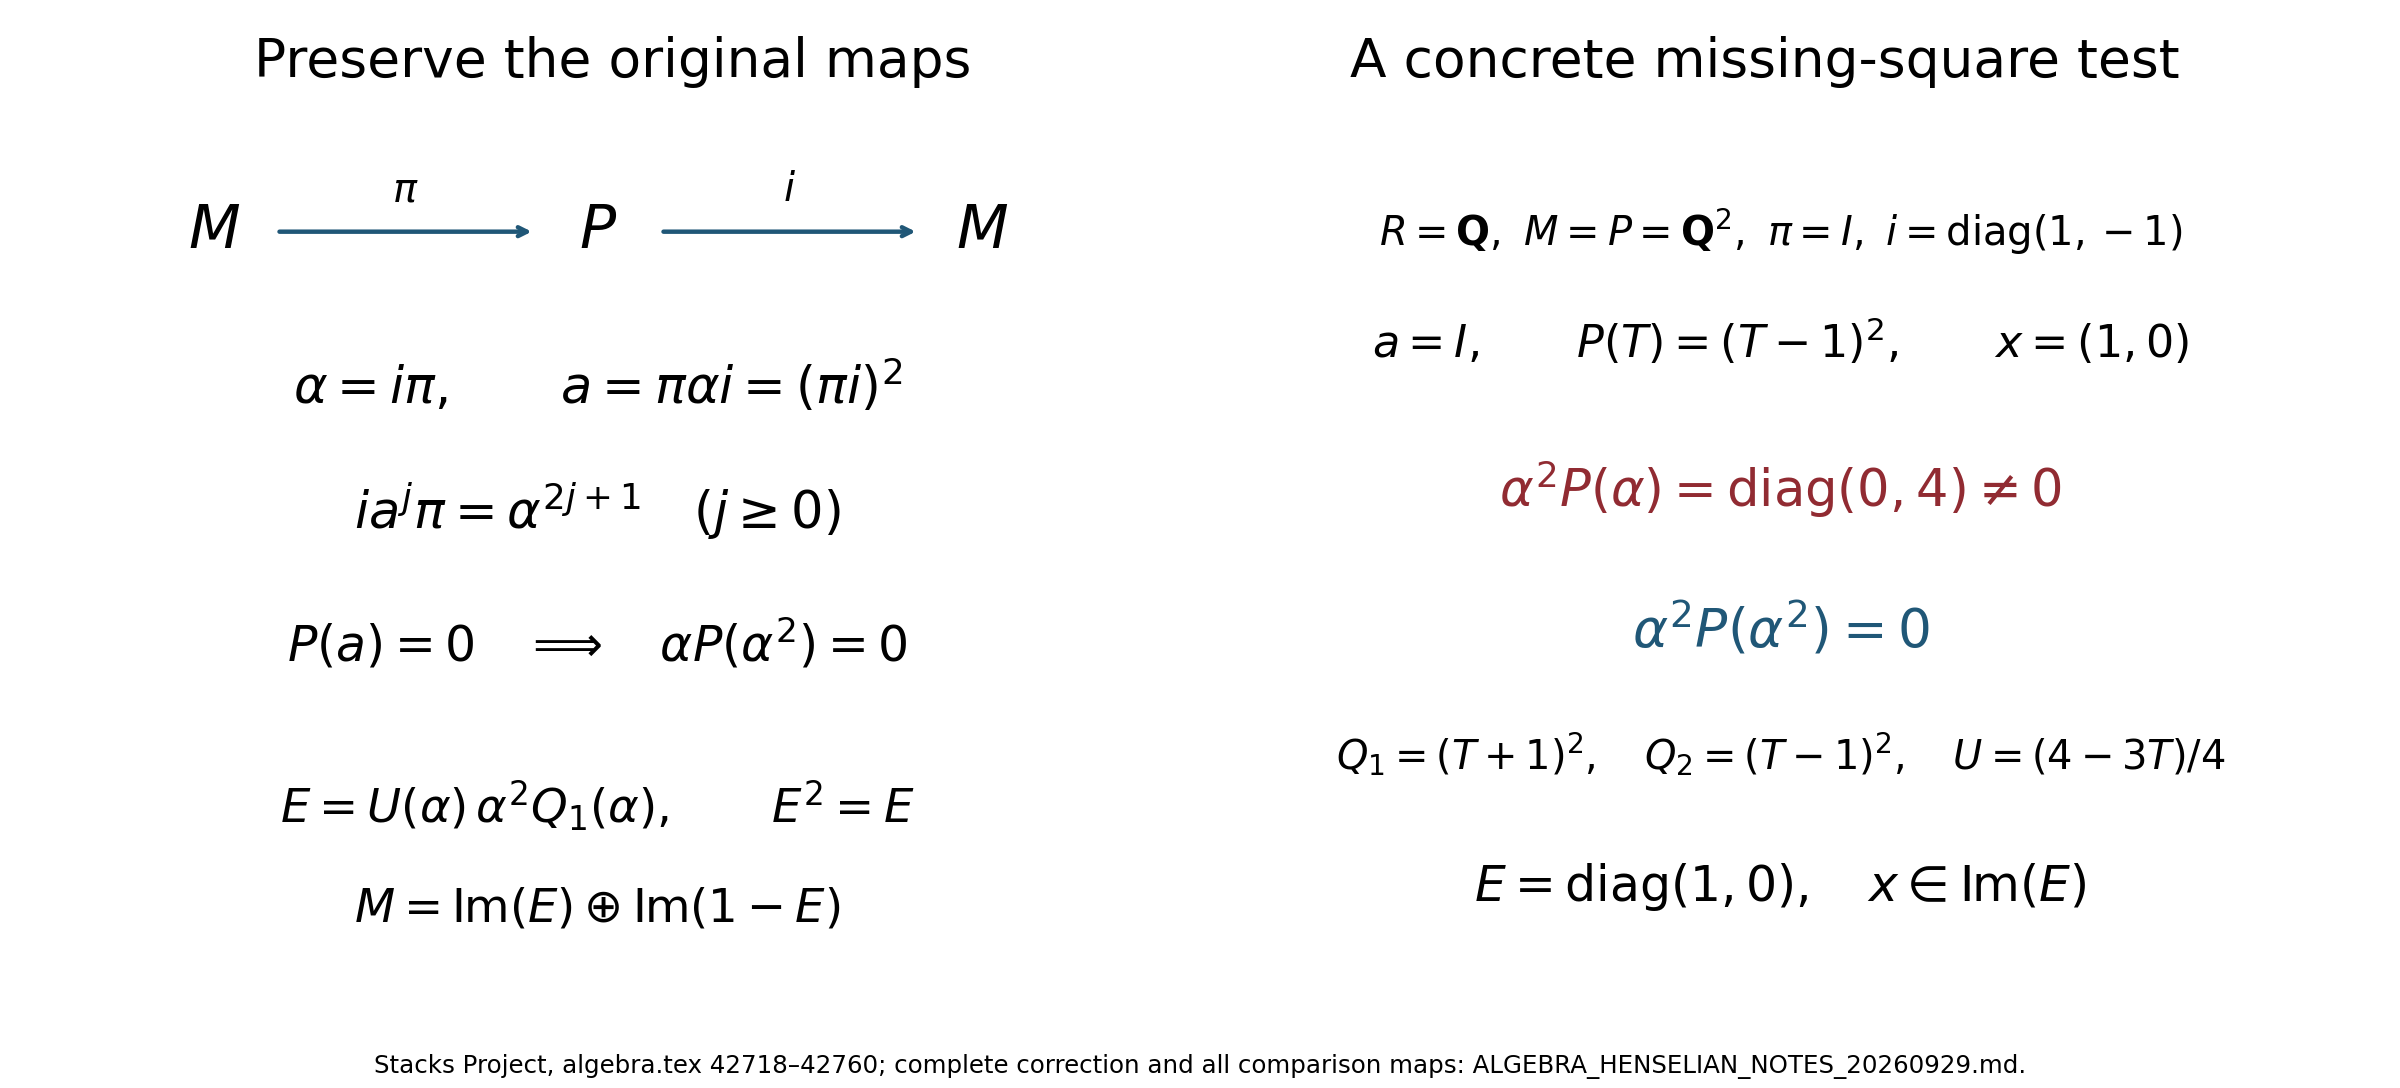
\includegraphics[keepaspectratio,alt={The original factorization and the corrected projection}]{HENSELIAN_PROJECTION_20260929.png}}
\caption{The original factorization and the corrected projection}
\end{figure}

The left panel records the original maps in the preceding proof. The right panel keeps the same rational counterexample and displays its corrected projection. Here the complete factors and coefficients are \[
A(T)=T^2(T+1)^2,\qquad B(T)=(T-1)^2,\qquad
U(T)=\frac{4-3T}{4},\qquad
V(T)=\frac{3T^3+8T^2+8T+4}{4}.
\] Indeed \[
4U(T)A(T)=-3T^5-2T^4+5T^3+4T^2,
\quad
4V(T)B(T)=3T^5+2T^4-5T^3-4T^2+4,
\] so their sum is exactly 4. Thus the displayed Bezout identity holds with every coefficient retained. Evaluation at the original \(\alpha=\operatorname{diag}(1,-1)\) gives \(A(\alpha)=\operatorname{diag}(4,0)\), \(B(\alpha)=\operatorname{diag}(0,4)\), and \(E=\operatorname{diag}(1,0)\). In particular the chosen fixed vector lies in the first summand. This is an illustration of the proved correction, with no change of the source's endomorphisms. Source: the Stacks Project authors, authority algebra.tex 42718--42760; the complete corrected argument is in the preceding section. Reproducible figure source: draw\_henselian\_projection\_20260929.py; vector edition: HENSELIAN\_PROJECTION\_20260929.svg. The PNG was inspected for legibility, exact formulas and arrow directions.

\subsubsection{Report dispositions and propagation}\label{report-dispositions-and-propagation}

The fourteen reports form eleven report groups. Seven source-correction units result after adding the independently found missing-square correction: eleven operations in total. The inverse-image orientation and product index are repaired; the residue polynomial and positive exponent are clarified; both zero-factor cases and the degree qualification are repaired; the undefined reference is replaced by lemma-mop-up. The module-polynomial letter reuse and the tensor-map name remain optional style changes. The quotient-polynomial scope convention, contraction notation and the true finite-étale-over-S assertion are not mathematical defects and are rejected as such.

The missing-square correction is propagated through all four uses of the annihilating relation, the lifted factors, both image summands, the actual surjection from the original finite module and the countable direct-sum proof. The finite-family projection is a proved consequence of that corrected construction. Separate editorial groups record complete and nil-ideal lifting, the finite-presentation boundary for general nil-ideal formal étale lifting, and the stronger Hom-set statement allowing every local target of a strictly henselian base. All remain visibly separate from the translated original. The broader synthesis and any mathematical paper remain after the core integration work.
